\documentclass[conference]{IEEEtran}
\IEEEoverridecommandlockouts
% The preceding line is only needed to identify funding in the first footnote. If that is unneeded, please comment it out.
\usepackage{cite}
\usepackage{amsmath,amssymb,amsfonts}
\usepackage{algorithmic}
\usepackage{graphicx}
\usepackage{textcomp}
\usepackage{xcolor}
\usepackage{float}
\def\BibTeX{{\rm B\kern-.05em{\sc i\kern-.025em b}\kern-.08em
    T\kern-.1667em\lower.7ex\hbox{E}\kern-.125emX}}
\begin{document}

\title{Recommendation ranking based on online comment mining and sentiment analysis
% \\
% {\footnotesize \textsuperscript{*}Note: Sub-titles are not captured in Xplore and
% should not be used}
% \thanks{Identify applicable funding agency here. If none, delete this.}
}
\author{
\IEEEauthorblockN{Hongyi Huang}
\IEEEauthorblockA{\textit{CCNU-UOW Joint-Institude} \\
\textit{Central China Normal University}\\
Wuhan, China \\
hongyi@gmail.com}
\and
\IEEEauthorblockN{Wangzhihui Mei}
\IEEEauthorblockA{\textit{CCNU-UOW Joint-Institude} \\
\textit{Central China Normal University}\\
Wuhan, China \\
maywzh@gmail.com}
\and
\IEEEauthorblockN{Yueyue He}
\IEEEauthorblockA{\textit{CCNU-UOW Joint-Institude} \\
\textit{Central China Normal University}\\
Wuhan, China \\
yueyue@gmail.com}
\and
\IEEEauthorblockN{Liting Lyu}
\IEEEauthorblockA{\textit{CCNU-UOW Joint-Institude} \\
\textit{Central China Normal University}\\
Wuhan, China \\
liting@gmail.com}

}

\maketitle

\begin{abstract}
    With the wide application of deep learning in recommendation system, a variety of algorithms are used in different reviews and recommendations. The traditional recommendation algorithm has no such method as using CNN or RNN models to do emotional analysis of text and using user behavior profiles such as collaborative filtering, which has become the mainstream. However, the effect of using text classification recommendation alone can not extract the potential features of text compared with emotional analysis. Based on the data of tourism review, the data variance is too large. For example, tourism experts will have 40-50 tourist reviews of scenic spots. The average user's comments on less than 10 sites are close to one or two. If the collaborative filtering algorithm is used for recommendation, the user matrix is too sparse to accurately describe the user profile. In view of this phenomenon, this paper uses CNN + attention + Rocchio to extract emotional feature values, and uses attention to extract and classify text details. Rocchio algorithm is used to rank and recommend scenic spots..
\end{abstract}

% \begin{IEEEkeywords}
% component, formatting, style, styling, insert
% \end{IEEEkeywords}

\section{Introduction}
With the rapid development of the Internet, more and more users choose to use the online tourism platform and the services provided by the tourism community, such as hotels, transportation, scenic spots tickets, etc. to carry out tourism planning. Some existing research results show that when consumers purchase goods or services, they usually browse the relevant reviews of the corresponding products or services \cite{1,2}.But when users browse the relevant historical information, they are faced with the problems of invalid comments and mixed comments.At the same time, the emotional intensity in historical reviews also affects users' judgment of products and services. For example, when users browse hotel related reviews, the emotional intensity revealed in the reviews, such as good, good, general, poor, poor, etc., will affect users' cognition of hotel services and then affect their choice.Not only that, different tourism platforms have different scores for the same tourism location, but also different evaluation dimensions and contents for the same tourism location, which makes it impossible for users to obtain complete information about a tourism destination from the same tourism platform, increasing the time cost and decision-making difficulty of user selection.Therefore, how to integrate the comment information of different tourism platforms on the same scenic spot across platforms, extract the theme features that users pay attention to, calculate the preference intensity of each feature, analyze the emotional intensity under the corresponding theme features and rate them, and finally generate the comprehensive rating of scenic spots and make a reasonable ranking is the practical problem of this study.

Based on user's comment information, this study uses LDA (topic extraction model) to extract features of scenic spots, and introduces attention mechanism model to get user's preference intensity for features of scenic spots. At the same time, convolution neural network technology is used to do emotional analysis for comments with the same features, extract the emotional intensity rating of features of main topics, and establish a recommendation ranking model integrating deep learning and emotional analysis It aims to integrate the user's historical information and provide users with reasonable scenic spot ranking recommendations, and solve the problem of information asymmetry and inconsistency among multiple platforms.



\subsection{Related Work}

\subsubsection{Research on attention mechanism based on deep learning}
As for the definition of attention mechanism, Turney P D et al. believe that attention mechanism is a model that simulates human brain's attention introduced from cognitive psychology. It can quickly lock the key points of the target from the massive information and eliminate the useless information to complete the task efficiently\cite{7}. The effective use of attention mechanism can help to analyze the user's preference for scenic spot features, and provide data basis for getting reasonable ranking recommendation. Based on neural network and attention mechanism, Gao Chengliang and others designed a bidirectional LSTM model combining part of speech information, which can easily learn implicit feature information from words and parts of speech, and improve the effect of text classification\cite{8}. The comprehensive rating of tourist attractions is mainly based on the user comments of the scenic spots on various platforms. Through the extraction and analysis of user comments, users' responses to different features of the scenic spots can be obtained. In terms of sequence model, Kang WC et al. put forward a sequence model based on self-attention, combining the advantages of RNN model and MC model, making the model superior to the most advanced sequence model\cite{9}. After getting the comprehensive score of each scenic spot, combining with the application of the model, the final ranking results can be optimized to achieve better recommendation effect.

In recent years, the recommendation system is gradually combined with deep learning to optimize the model and improve the prediction effect. In the study of neural network based on attention mechanism, Li J et al. explored a hybrid encoder with attention mechanism to model the user's sequential behavior, capture the main purpose of the user in the current session and calculate the rating, so as to optimize the model. Experiments show that the neural attention recommendation machine has a strong recommendation effect\cite{10}. In the application of scenic spot recommendation, the coder models the user's order behavior of browsing the tourism platform, analyzes the user's tourism preference and carries out rating. C these studies are based on attention mechanism and deep learning, and play a role in different levels of the recommendation system which integrates attention mechanism, which can significantly improve the prediction effect of the model.

\subsubsection{Sentiment analysis based on convolutional neural network}
Sentiment analysis also known as opinion mining or opinion analysis, was first proposed by Nasukawa \cite{10} et al. in 2003. Its purpose is to analyze users' positive, negative or middle feelings towards entities and their attributes through data mining.

Convolution neural network is a kind of feedforward neural network with convolution calculation and depth structure. It is one of the representative algorithms of depth learning. It is widely used in image recognition, natural language processing and other fields. According to the existing research, convolutional neural network has a good effect in the emotional analysis of text data. Li Hui and Cai Yaqing proposed a fine-grained sentiment analysis method based on convolutional neural network, and found that compared with traditional sentiment classification model and conventional CNN model, this method improved the accuracy, recall rate and F-score evaluation index\cite{4}; Wang Yuhan and Zhang Chunyun used word 2vec method to initialize text sub vector, and used CNN model to learn deep semantic information in text Finally, we can find out the emotional tendency of twitter text \cite{5}; He Hongye, Zheng Jin, et al. use part of speech features to catch the polysemy phenomenon of text which can't be recognized by traditional word vectors, and combine with the original representation method of input text to construct a two-channel input of convolutional neural network, and build a text convolutional neural network model combining part of speech features\cite{7}; Wang Wenkai, Wang Liming et al. constructed a microblog emotion analysis model based on convolutional neural network, and proved that the model has excellent characteristics in microblog emotion analysis \cite{8}. All the above studies have proved the feasibility of using convolutional neural network model to analyze text emotion.

After the analysis of the existing literature, we can see that although the existing research has the subject feature extraction of text analysis, there is the integration of attention mechanism into the recommendation model, but it is less to extract the subject words from online comments, and for multi-platform.

To sum up, in the field of recommendation service research, the topic feature extraction, attention mechanism and convolution neural network of text analysis have been studied in depth respectively, but there are not many researches on the fusion of the three, cross platform online comments and travel location ranking recommendation. Therefore, this study proposes a kind of scenic spot ranking recommendation, which integrates deep learning and emotional analysis, to provide practical help for users to choose scenic spots.

\subsection{Organization of this paper}
In the second part of this paper, the relevant background is briefly introduced. The third part is a brief description of the related technologies designed in this paper. The fourth part describes the research methods. In the fifth part of this paper, we describe the system we do. In the sixth part, it makes a summary.

\section{preliminaries}

\subsection{CNN}
Convolutional Neural Networks (CNN) is a kind of Feedforward Neural Networks that contains Convolutional computation and has a deep structure. It is one of the representative algorithms of deep learning. The convolutional Neural network has the capability of representation learning, and can carry out shift-invariant classification of input information according to its hierarchical structure. Therefore, it is also known as "shift-invariant Artificial Neural Networks (SIANN)".

The research on convolutional neural networks began in the 1980s and 1990s. Time-delay network and lenet-5 were the first convolutional neural networks. After the 21st century, with the development of deep learning theory and the improvement of numerical calculation equipment, convolutional neural network has developed rapidly and been applied to computer vision, natural language processing and other fields.

Convolution neural network imitation biological visual perception, visual perception mechanism building, can undertake supervised learning and unsupervised learning, the convolution kernel parameters of sharing in the underlying layer and interlayer connection of sparse sex enables the convolutional neural network to the smaller amount of calculation was (grid - like the topology) characteristics, such as pixels and audio learning, with stable effect and characteristics of data without additional engineering (feature engineering) requirements.

\subsection{Attention}
The Attention Mechanism stems from the study of human vision. In cognitive science, because of bottlenecks in information processing, humans selectively focus on one part of all information while ignoring other visible information. These mechanisms are often referred to as attentional mechanisms. A different part of the human retina have different levels of information processing ability, namely the Acuity, the only central retinal concave part has the strongest Acuity. In order to make rational use of limited visual information processing resources, humans need to select a specific part of the visual area and focus on it. For example, when people are reading, usually only a few words to be read are paid attention to and processed. To sum up, attention mechanism mainly has two aspects: deciding which part of input needs to be paid attention to; Allocate limited information processing resources to important parts.

An informal term for attentional mechanisms is that neural attentional mechanisms enable neural networks to focus on a subset of their inputs (or characteristics): the selection of specific inputs. Attention can be applied to any type of input regardless of its shape. In the case of limited computing capacity, the attention mechanism is a resource allocation scheme which is the main means to solve the problem of information overload, allocating computing resources to more important tasks.

Attention is generally divided into two types: one is top-down conscious attention, called focus. Focused attention refers to the attention that has a predetermined purpose, depends on the task, and focuses on a certain object actively and consciously. The other is bottom-up unconscious attention, called saliency-based attention. Attention based on significance is attention driven by external stimuli, does not require active intervention, and is irrelevant to the task. If an object's stimulus information is different from the surrounding information, an unconscious winner-take-all or gating mechanism can direct attention to the object. Whether this attention is intentional or not, most brain activity relies on attention, such as remembering information, reading or thinking.

In cognitive neuroscience, attention is a complex cognitive function indispensable to human beings. It refers to the ability to choose to pay attention to some information while ignoring others. In daily life, we receive a large amount of sensory input through visual, auditory, tactile and other means. But our brains are able to work methodically in the midst of this onslaught of information, because they can consciously or unconsciously choose small pieces of useful input to focus on and ignore the rest. This ability is called attention. Attention can be either external stimuli (hearing, sight, taste, etc.) or internal consciousness (thinking, remembering, etc.).

\subsection{Riochho}
Rocchio algorithm is a method to modify the original query through the initial matching document of the query in IR to optimize the query.

The basic idea is to construct a prototype vector for each class by using training set. The construction method is as follows:
Given a class, all the components of the corresponding vectors of the documents belonging to this class in the training set are represented by positive numbers, and the components of the corresponding vectors of the documents not belonging to this class are represented by negative numbers. Then all the vectors are added up, and the resulting sum vector is the prototype vector of this class. The similarity of the two vectors is defined as the cosine of the angle between the two vectors, and the training set is calculated one by one The similarity of all documents and prototype vectors, and then select a certain similarity as a boundary according to a certain algorithm. Given a document, if the similarity between this document and the prototype vector is large, then this document belongs to this class, otherwise this document does not belong to this class. The outstanding advantage of Rocchio algorithm is that it is easy to implement, and the calculation (training and classification) is particularly simple. It is usually used to implement the benchmark system to measure the performance of classification system.


\section{Research method}
The research method in this paper mainly extracts sentiment rating and generates sentiment feature Si by obtaining a large number of data sets and training CNN with manually annotated data. At the same time, attention model was used to extract the subject word Mi of the same data. These two parameters are used to enter the sorting algorithm and update the manually labeled scenic spot feature values. In the research, the efficiency and accuracy of the two algorithms are compared with other algorithms under the same working conditions. The recommendation accuracy of the recommendation system is tested by the actual score on the website. The Figure 1 is the flow chart of the whole process. First, we manually annotate the data set and take manual annotation for scenic spots < tag1,tag2....tagn > , which USES the data set for training word2vec. After training word2vec, It was used to obtain the feature vector Fi and the emotion rating Si marked in the data set and output it to CNN. In the process of CNN training, the necessary convolution kernel, pooling layer and hidden layer are designed. After that, the trained CNN is saved to output emotion rating Si. At the same time, input Fi into attention model and specify the generated sequence < tag1,tag2....tagn > to achieve the effect of seq2seq. Determine whether there is a tagi. If there is no tag, The overall score might decrease accordingly\cite{7}.

\section{Our work}
\subsection{Data processing}
The data set is the review data on travel websites such as hornet's nest, ctrip and tuniu. LabeledTrainData is required for text classification, but unlabeled data can be used together when training word2vec word vector model (unsupervised learning). after a word2vec product a the X matrix into the CNN and Attention model.
\begin{figure}[H]
    \centering
    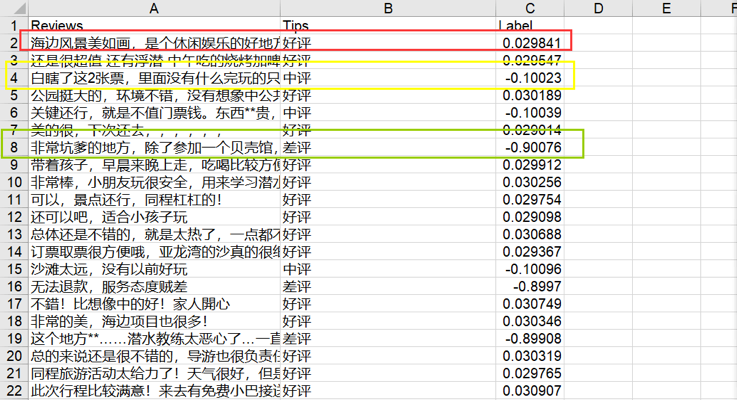
\includegraphics[width=0.8\linewidth]{figure/Picture1}
    \caption{Data set}
\end{figure}


\subsection{Attention model}
BI-LSTM + Attention is to add an Attention layer to the model of BI-LSTM . InBI-LSTM , useing the output vector of the last sequence as the feature vector, and then conduct softmax classification. Attention is to calculate the weight of each sequence first, then add all the vectors of the sequence as eigenvectors, and then conduct softmax classification. In the experiment, adding Attention did improve the results. The model structure is as Fig.2:
\begin{figure}[H]
    \centering
    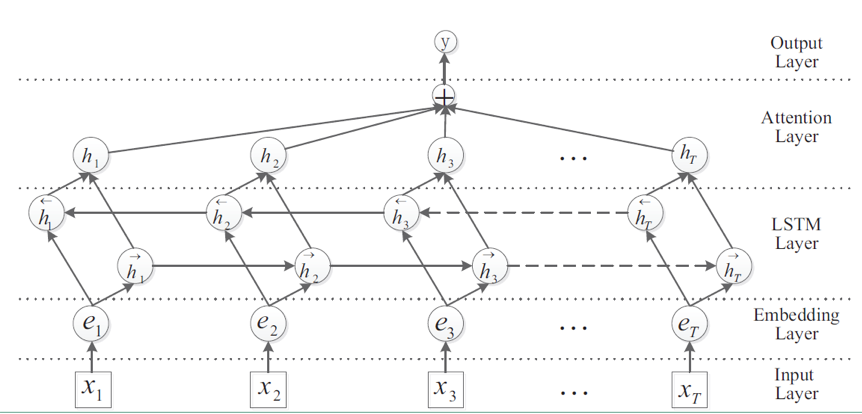
\includegraphics[width=0.8\linewidth]{figure/Picture2}
    \caption{Structure of Attention model}
\end{figure}


\begin{enumerate}
    \item Input layer: input sentence to this model; 
    \item Embedding layer: map each word into a low dimension vector; 
    \item LSTM layer: utilize BLSTM to get high level features from step 2; 
    \item Attention layer: produce a weight vector, and merge word-level features from each time step into a sentence-level feature vector, by multiplying the weight vector; 
    \item (5) Output layer: the sentence-level feature vector is finally used for relation classifification. 
    In the first step using the X which word2vec produced. Into the input layer ,then Embedding it get a $e_i$ the ei in to the LSTM layer which might help to the time sequence.
\end{enumerate}
After the LSTM Layer the $h_i$ into the softmax to get a output $tag_i$

\subsection{CNN Model}
Analyze the emotional tendency of the comment on the subject characteristics
In the field of natural language, the function of convolution is to capture the emotion of the comment text by using the local characteristics of the text. The convolution neural network used in this study is composed of word vector mapping layer, convolution layer, pooling layer, full connection layer and softmax layer. The cleaned comment sets containing subject features are processed into word vectors with sentences as a sample unit. Based on the word feature representation proposed in this paper, the words related to emotional tags are further extracted through the convolution layer and pooling layer Through the full connection layer and softmax layer, we get the emotion rating vector of the user to the theme feature F.

\subsection{rating based on preference and emotional intensity of theme characteristics}
The user's decision on a scenic spot depends on the user's characteristic preference and emotional tendency. Therefore, this study integrated theme preference and emotional intensity to rank. The rating results are as follows:

\begin{figure}[H]
    \centering
    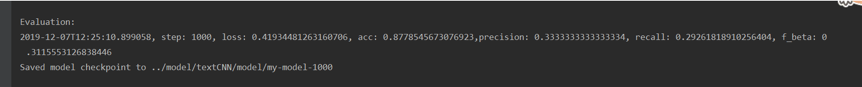
\includegraphics[width=0.8\linewidth]{figure/Picture3}
    \caption{Results}
\end{figure}


In this paper, the $tag_i$ obtained from attention and the $f$ obtained from CNN are taken as parameters, the specific tag in tag n is updated. If no tag can be extracted from the comment, we set $tag_n$ to NUT (Unkonw tag)

$$U_{o p t}=\operatorname{argmax}\left[\operatorname{sim}\left(U_{c}, V_{1}-\operatorname{Sim}\left(U_{c}, V_{h}\right)\right)\right]$$

$$U_{opt}=\alpha U_0+\beta \frac{1}{|V_1|}\sum_{\vec{w_j}\in V_1}{\vec{w_j}}-\gamma\frac{1}{|V_h|}\sum_{\vec{w_j}\in V_h}{\vec{w_j}}$$

$V_L$ represents the type the user likes, $V_h$ represents the type the user hates, and $sim$ represents the user likes similarity and USES cosine similarity.



\section{Conclusion}
After the above processing, we can conduct emotion analysis and text classification on the sparse comment data set of user matrix. And the scenic spots are evaluated based on classification and analysis to avoid the imprecise push caused by the use of collaborative filtering algorithm. And the accuracy of emotion analysis and text classification can not be matched by a single model.

\begin{thebibliography}{00}
\bibitem{1} G. Eason, B. Noble, and I. N. Sneddon, ``On certain integrals of Lipschitz-Hankel type involving products of Bessel functions,'' Phil. Trans. Roy. Soc. London, vol. A247, pp. 529--551, April 1955.
\bibitem{2} J. Clerk Maxwell, A Treatise on Electricity and Magnetism, 3rd ed., vol. 2. Oxford: Clarendon, 1892, pp.68--73.
\bibitem{3} I. S. Jacobs and C. P. Bean, ``Fine particles, thin films and exchange anisotropy,'' in Magnetism, vol. III, G. T. Rado and H. Suhl, Eds. New York: Academic, 1963, pp. 271--350.
\bibitem{4} K. Elissa, ``Title of paper if known,'' unpublished.
\bibitem{5} R. Nicole, ``Title of paper with only first word capitalized,'' J. Name Stand. Abbrev., in press.
\bibitem{6} Y. Yorozu, M. Hirano, K. Oka, and Y. Tagawa, ``Electron spectroscopy studies on magneto-optical media and plastic substrate interface,'' IEEE Transl. J. Magn. Japan, vol. 2, pp. 740--741, August 1987 [Digests 9th Annual Conf. Magnetics Japan, p. 301, 1982].
\bibitem{7} M. Young, The Technical Writer's Handbook. Mill Valley, CA: University Science, 1989.
\bibitem{8} Wenpeng Yin, Hinrich Schutze, Bing Xiang, and Bowen Zhou. Abcnn: Attention-based convolutional neural network for modeling sentence pairs. Transactions of the Association for Computational Linguistics, 4:259–272, 2016. 
\bibitem{9} Tom Young, Devamanyu Hazarika, Soujanya Poria, and Erik Cambria. Recent trends in deep learning based natural language processing. ieee Computational intelligenCe magazine, 13(3):55–75, 2018. 
\bibitem{10} Fei Yu, An Zeng, S ́ebastien Gillard, and Matu ́ˇs Medo. Network-based recommendation algorithms: A review. Physica A: Statistical Mechanics and its Applications, 452:192–208, 2016. 
\end{thebibliography}

% \bibliography{ref}
% \vspace{12pt}
% \color{red}
% IEEE conference templates contain guidance text for composing and formatting conference papers. Please ensure that all template text is removed from your conference paper prior to submission to the conference. Failure to remove the template text from your paper may result in your paper not being published.

\end{document}
